\newpage






%\begin{figure}[!b]
%    \begin{center}
%        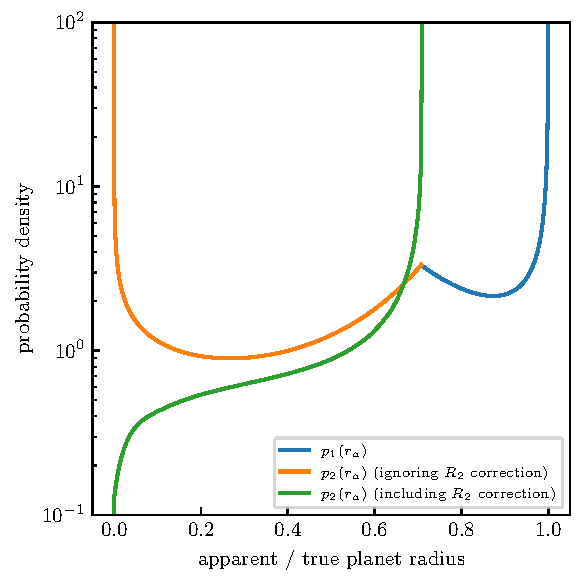
\includegraphics[width=.9\textwidth]{figures/prob_r_a.pdf}
%    \end{center}
%    \caption{Model \#2 (Sec.~\ref{sec:model_2}): 
%    probability of observing an apparent radius $r_a$ given a 
%    planet orbiting the primary, $p_1(r_a)$, or the secondary, $p_2(r_a)$ of 
%    a 
%    binary system.
%    The true planet radius is fixed~--~a delta function centered on ``1''.
%    This plot takes $\alpha=3.5, \beta=0$, for $\alpha$ the exponent in 
%    the mass-luminosity relation $L \propto M^\alpha$, and $\beta$ the 
%    exponent in the distribution of mass ratios in a volume-limited sample.
%    Each distribution is separately normalized.
%    }
%    \label{fig:model2_prob_r_a}
%\end{figure}
